\chapter{Multipath Analysis}

\section{2-Ray Model}
The 2-Ray multipath model over a flat earth is given in Figure \ref{mp_fig:1}. In this figure, $P_1$ and $P_2$ are the two points we are interested in propagating between and $P_2'$ is the mirror image of $P_2$. $L_1$ is then the direct path and $L_{so}$ represents the shortest orbit reflection from the sea surface. The altitudes of the two points from the mean sea surface are $h_1$ and $h_2$, the total downrange distance is $L$, and the distance to the reflection point is $x_m$.

\begin{figure}[H]
  \begin{center}
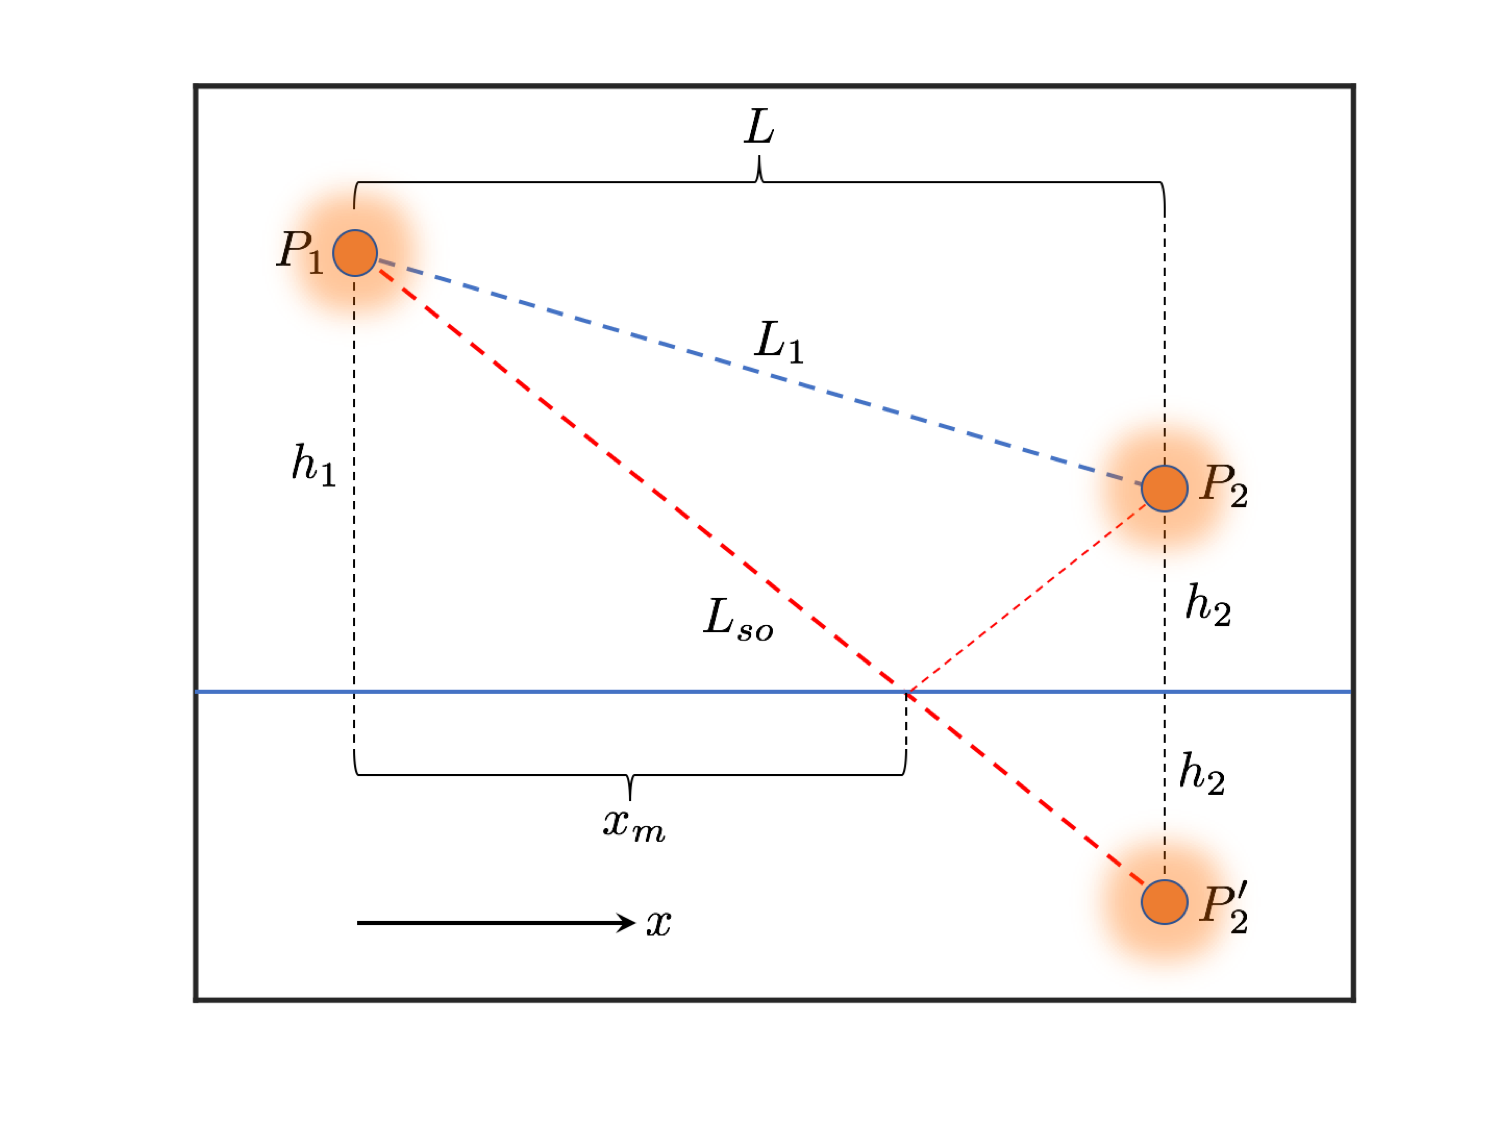
\includegraphics[width=5in]{../media/analysis/multipath_2_ray.png}
  \end{center}
  \renewcommand{\baselinestretch}{1} \small\normalsize
  \begin{quote}
    \caption[2 Ray Multipath Geometry]{ 2 Ray Multipath Geometry\label{mp_fig:1}}
  \end{quote}
\end{figure}
\renewcommand{\baselinestretch}{2} \small\normalsize

To capture the effects of propagating over a spherical earth, the altitude $h_2$ can be modified with a correction factor \cite{blake_radar} dependent on the effective radius of the earth, $r_e = (4/3) 6,371,000$ m.
\begin{equation}
h_2' = h_2 - \frac{L^2}{2r_e}
\label{mp_eq:0}
\end{equation}

The path lengths are given by geometry and simplified through a binomial expansion.
\begin{equation}
\begin{aligned}
L_1 & = \sqrt{L^2 + (h_1-h_2)^2}  \approx L + \frac{(h_1 - h_2)^2}{2L}\\
L_{so} & = \sqrt{L^2 + (h_1+h_2)^2}  \approx L + \frac{(h_1 + h_2)^2}{2L}\\
\end{aligned}
\label{mp_eq:1}
\end{equation}
\renewcommand{\baselinestretch}{2} \small\normalsize

From Huygen's principle, the propagation factor for the 2-ray model is the sum of plane waves traveling along the paths $L_1$ and $L_{so}$. Here $\Gamma_1$ is the reflection coefficient from the sea surface, $\Gamma_1 = \Gamma(x_m)$.
\begin{equation}
\boxed{F_p = e^{ikL_1} + \Gamma_1e^{ikL_{so}}}
\label{mp_eq:1b}
\end{equation}

We can now look at the phase difference between the two primary paths, $\Delta\varphi = k\left[ L_1 - L_{so}\right]$.
\begin{equation}
\boxed{\Delta\varphi = -\frac{4\pi h_1h_2}{\lambda L}}
\label{mp_eq:7}
\end{equation}
\renewcommand{\baselinestretch}{2} \small\normalsize

\noindent The derivative of the phase difference with respect to range is then
\begin{equation}
\frac{d\Delta\varphi}{dL}=-\frac{4\pi h_1h_2}{\lambda L^2}
\label{mp_eq:8}
\end{equation}

\noindent This can be converted from rad/m to rad/sample by multiplying by the spatial sampling distance in range, $\Delta L$. We can insist that this phase shift per sample be smaller than some pre-determined value to provide adequate sampling. It is often convenient to specify a limit in terms of wavelengths and we can enforce the condition that there must be at least $n$ samples per wavelength by letting

\begin{equation}
\frac{4\pi h_1h_2\Delta L}{\lambda L^2} \leq \frac{2\pi \lambda}{n}
\label{mp_eq:10}
\end{equation}

This yields a constraint for the maximum allowable spatial sampling step to ensure $n$ samples per wavelength.
\begin{equation}
\boxed{\Delta L \leq \frac{\lambda^2 L^2}{2nh_1h_2}}
\label{mp_eq:11}
\end{equation}

\section{Multiple Ray Model}
To include multiple rays, we must consider the region over which the electromagnetic wave reflects from the surface, $\tilde{x}$, as shown in Figure \ref{mp_fig:2}. This figure extends Figure \ref{mp_fig:1}, and  $L_2$ and $L_3$ are the path lengths for the various reflected rays and $s(x)$ is the altitude of the sea surface at $x$. 

\begin{figure}[H]
  \begin{center}
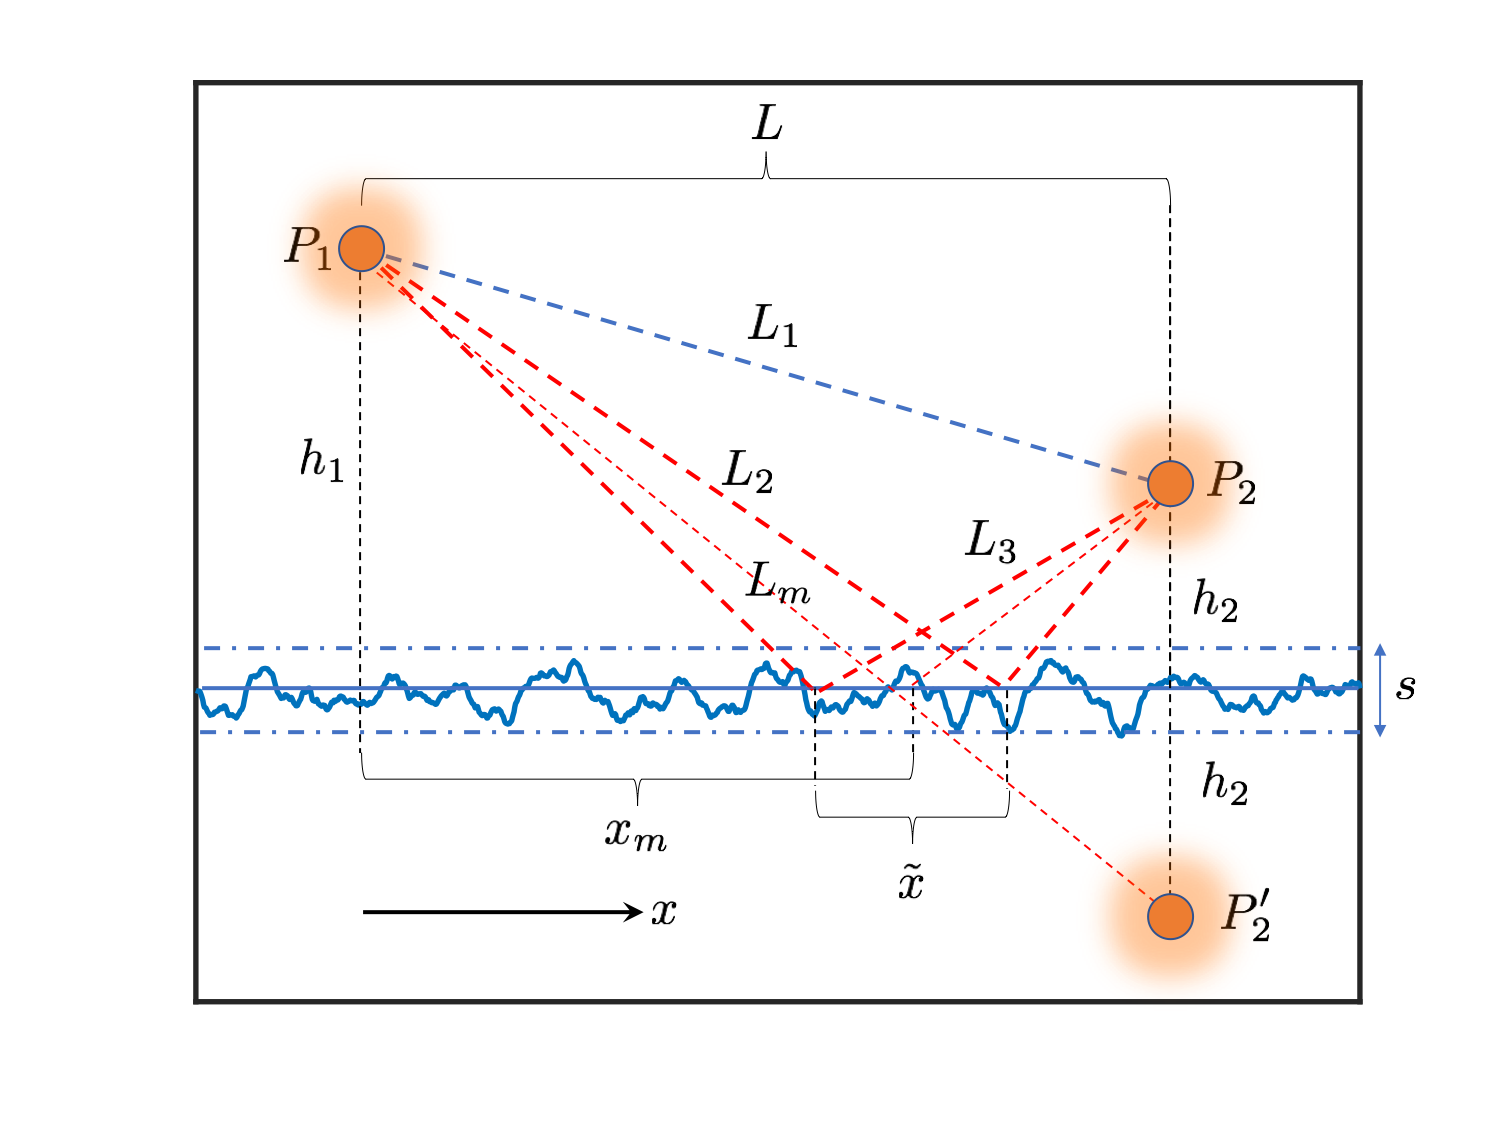
\includegraphics[width=5in]{../media/analysis/multipath_layout.png}
  \end{center}
  \renewcommand{\baselinestretch}{1} \small\normalsize
  \begin{quote}
    \caption[Multipath Geometry with Random ]{ Multipath Geometry\label{mp_fig:2}}
  \end{quote}
\end{figure}
\renewcommand{\baselinestretch}{2} \small\normalsize


The path lengths  $L_2$ and $L_3$ can be defined through similar triangles around $x$ and can again be simplified through a binomial expansion. At high altitudes or small sea states, $2h_1s(x) >> s^2(x)$ and we can neglect the $s^2(x)$ term.
\begin{equation}
\begin{aligned}
L_2 &= \sqrt{x^2 + \left( h_1 - s(x)\right)^2}  \approx x + \frac{h_1^2-2h_1s(x)}{2x}\\
L_3 & = \sqrt{\left(L - x\right)^2 + \left( h_2 - s(x)\right)^2}  \approx L-x + \frac{h_2^2 - 2h_2s(x)}{2\left(L-x\right)}\\
\end{aligned}
\label{mp_eq:12}
\end{equation}
\renewcommand{\baselinestretch}{2} \small\normalsize

The path length for a given reflected ray, $L_r$ is then given by
\begin{equation}
\begin{aligned}
L_r &= L_2 + L_3 \\
& = x + \frac{h_1^2-2h_1s(x)}{2x} +  L-x + \frac{h_2^2 - 2h_2s(x)}{2\left(L-x\right)} \\
& = L + \frac{1}{2}\left[\frac{h_1^2}{x} + \frac{h_2^2}{L-x} \right] - s(x)\left[ \frac{h_1}{x} + \frac{h_2}{L-x}\right] \\
&= L + L_0 - L_s
\end{aligned}
\label{mp_eq:13}
\end{equation}
\renewcommand{\baselinestretch}{2} \small\normalsize

Here $L_0$ represents the deterministic component due to reflection from the surface and $L_s$ represents the random component due to reflection from the surface. The reflection point from the 2-ray model, $x_m$, should be a saddle point and provide the dominant contribution. We can therefore perform a Taylor expansion of $L_0$ about $x_m$.

\begin{equation}
L_0 \approx L_0(x_m) + \frac{1}{2}\frac{d^2L_0}{dx^2}\bigg|_{x_m}(x-x_m)^2
\label{mp_eq:14}
\end{equation}

\begin{equation}
\frac{dL_0}{dx} = \frac{1}{2}\left[\frac{-h_1^2}{x^2} + \frac{h_2^2}{(L-x)^2} \right]
\label{mp_eq:15}
\end{equation}

\begin{equation}
\frac{d^2L_0}{dx^2} = \frac{h_1^2}{x^3} + \frac{h_2^2}{(L-x)^3} 
\label{mp_eq:16}
\end{equation}

Since $\frac{dL_0}{dx}\big|_{x_m} = 0$, we can solve for $x_m$
\begin{equation}
\begin{gathered}
\frac{-h_1^2}{x_m^2} + \frac{h_2^2}{(L-x_m)^2} = 0\\
\frac{-h_1}{x_m} + \frac{h_2}{L-x_m} = 0\\
\frac{h_1}{x_m} = \frac{h_2}{L-x_m}\\
h_1(L-x_m) = h_2x_m\\
x_m = \frac{h_1L}{h_1+h_2}
\end{gathered}
\label{mp_eq:17}
\end{equation}

This gives the following for the lowest Taylor series terms:

\begin{equation}
\begin{aligned}
L_0(x_m) &= \frac{(h_1+h_2)^2}{2L} \\
\frac{d^2L_0}{dx^2}\big|_{x_m}  &= \frac{(h_1+h_2)^4}{h_1h_2L^3} \\
L_s(x_m) &= \frac{2s(x)(h_1 + h_2)}{L}\\
\end{aligned}
\label{mp_eq:17a}
\end{equation}

The expansion of $L_0$ is then
\begin{equation}
L_0 \approx \frac{(h_1+h_2)^2}{2L} + \frac{(h_1+h_2)^4}{2h_1h_2L^3}(x-x_m)^2
\label{mp_eq:18}
\end{equation}

The propagation factor will now include all the reflections from the surface

\begin{equation}
\begin{aligned}
F_p &= e^{ikL_1} + \int_0^Ldx\Gamma  e^{ik(L_2+L_3)}\\
&= e^{ikL_1} + \int_0^Ldx\Gamma  e^{ik(L+L_0-L_s)}\\
&= e^{ikL_1} +  \Gamma_1e^{ik(L+\frac{(h_1+h_2)^2}{2L})}\int_0^Ldx\frac{\Gamma}{\Gamma_1} e^{ik(\frac{L_0''}{2}(x-x_m)^2-L_s)}\\
&= e^{ikL_1} + \Gamma_1e^{ikL_{so}}\int_0^Ldx\frac{\Gamma}{\Gamma_1} \exp\left[\frac{ikL_0''}{2}(x-x_m)^2 - \frac{i2ks(x)(h_1+h_2)}{L}\right]\\
\end{aligned}
\label{mp_eq:20}
\end{equation}

We have a similar expression to Equation \ref{mp_eq:1b} with the propagation factor from the shortest orbit reflection scaled by contributions from all the other reflected rays. letting $x-x_m \rightarrow \tilde{x}$, we can express the propagation factor as

\begin{equation}
\boxed{F_p = e^{ikL_1} + \Gamma_1 e^{ikL_{so}}\int_{-x_m}^{L-x_m}d\tilde{x} \frac{\Gamma(\tilde{x})}{\Gamma_1}\exp\left[\frac{ikL_0''}{2}\tilde{x}^2 - \frac{i2ks(\tilde{x})(h_1+h_2)}{L}\right]}
\label{mp_eq:21}
\end{equation}

\section{Asymptotic Approach for Deterministic Component}
For the deterministic component, we wish to solve the integral given by
\begin{equation}
I = \int_{-x_m}^{L-x_m}d\tilde{x} \frac{\Gamma(\tilde{x})}{\Gamma_1}\exp\left[\frac{ikL_0''}{2}\tilde{x}^2\right]
\label{mp_eq:22}
\end{equation}

The phase of the integrand oscillates rapidly as shown by the real part of the integrand in Figure \ref{mp_fig:3} with a 10m altitude target, Figure \ref{mp_fig:4} with a 20m altitude target and Figure \ref{mp_fig:5} with a 50m altitude target.

\begin{figure}[H]
  \begin{center}
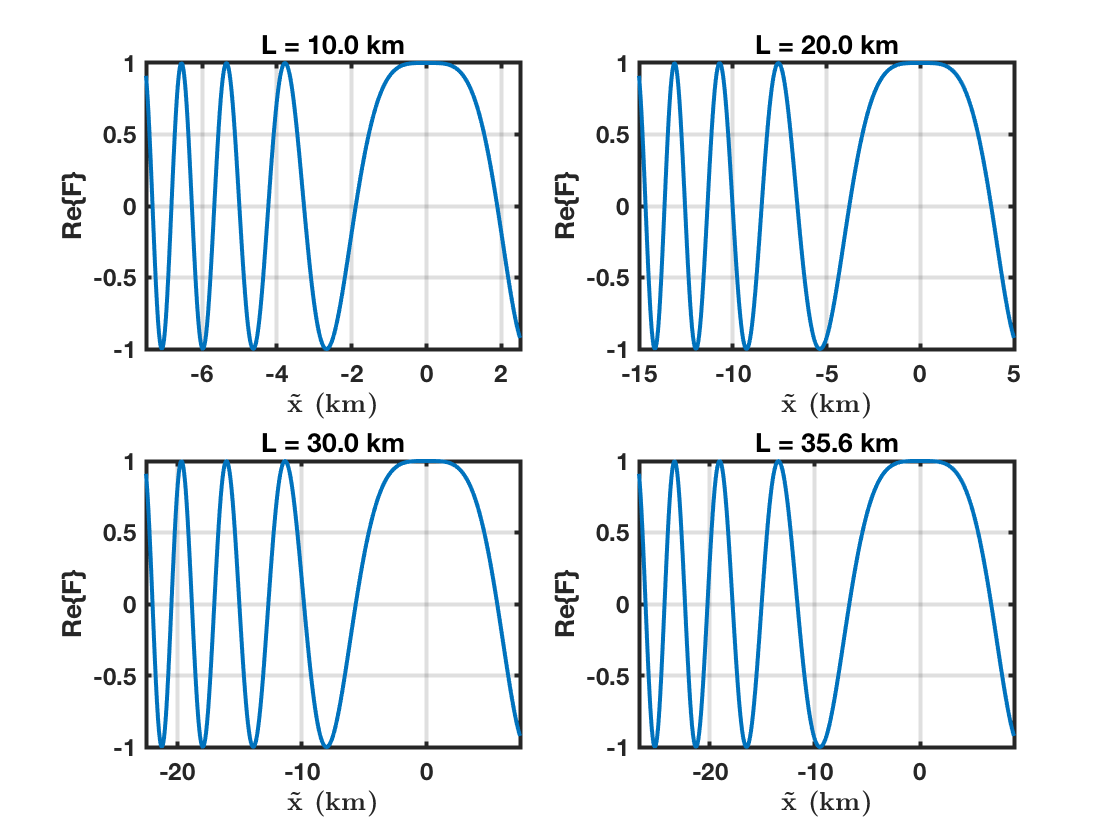
\includegraphics[width=4in]{../media/analysis/phaseVariation_30_10}
  \end{center}
  \renewcommand{\baselinestretch}{1} \small\normalsize
  \begin{quote}
    \caption[Real Part of Integrand for $h_1$ = 30m, $h_2$ = 10m]{ Real Part of Integrand for $h_1$ = 30m, $h_2$ = 10m\label{mp_fig:3}}
  \end{quote}
\end{figure}
\renewcommand{\baselinestretch}{2} \small\normalsize

\begin{figure}[H]
  \begin{center}
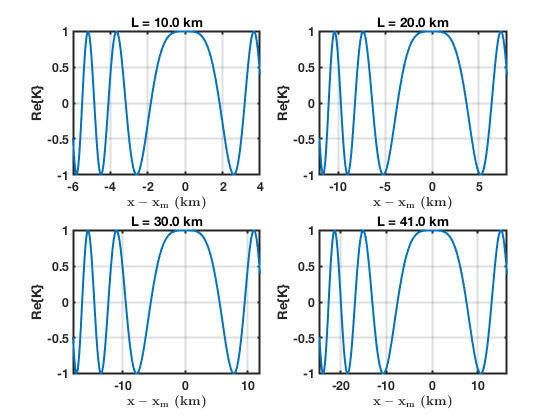
\includegraphics[width=4in]{../media/analysis/phaseVariation_30_20}
  \end{center}
  \renewcommand{\baselinestretch}{1} \small\normalsize
  \begin{quote}
  \caption[Real Part of Integrand for $h_1$ = 30m, $h_2$ = 20m]{ Real Part of Integrand for $h_1$ = 30m, $h_2$ = 20m\label{mp_fig:4}}
  \end{quote}
\end{figure}
\renewcommand{\baselinestretch}{2} \small\normalsize

\begin{figure}[H]
  \begin{center}
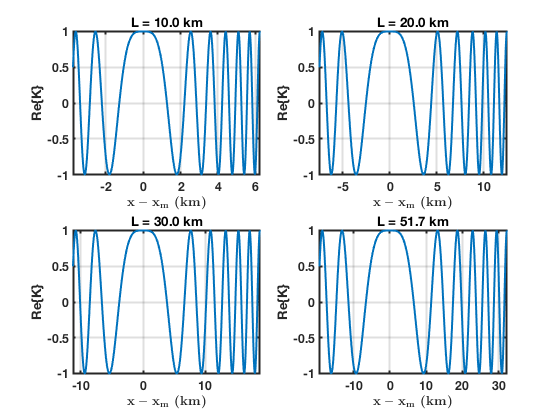
\includegraphics[width=4in]{../media/analysis/phaseVariation_30_50}
  \end{center}
  \renewcommand{\baselinestretch}{1} \small\normalsize
  \begin{quote}
  \caption[Real Part of Integrand for $h_1$ = 30m, $h_2$ = 50m]{ Real Part of Integrand for $h_1$ = 30m, $h_2$ = 10m\label{mp_fig:5}}
  \end{quote}
\end{figure}
\renewcommand{\baselinestretch}{2} \small\normalsize

Even with low altitudes, the phase oscillations will be rapid as $\tilde{x}$ goes past the limits of integration and will cancel out, so we can use the principle of stationary phase and let the limits of integration go to $\pm\infty$. Since the integrand is an even function, we can then take the limits from $0$ to $+\infty$ and multiply by 2.

\begin{equation}
I = \int_{-\infty}^{\infty}d\tilde{x} \frac{\Gamma(\tilde{x})}{\Gamma_1}\exp\left[\frac{ikL_0''}{2}\tilde{x}^2\right] = 2\int_{0}^{\infty}d\tilde{x} \frac{\Gamma(\tilde{x})}{\Gamma_1}\exp\left[\frac{ikL_0''}{2}\tilde{x}^2\right] 
\label{mp_eq:23}
\end{equation}

To solve this equation, we can work in the complex plane as shown in Figure \ref{mp_fig:6}. The contour along the real axis, $\mathcal{C}_1$, is deformed to ensure we do not cross through the singular point at $\tilde{x} = L-x_m$ as given in Equation \ref{mp_eq:13} for the initial expression of $L_0$. From Jordan's Lemma, the contour along the arc $\mathcal{C}_2$ will be $0$. Since there are no singular points enclosed by the contour, the sum of the integrals along the contours is $0$ so that

\begin{equation}
I = -2\int_{\mathcal{C}_3}d\tilde{x} \frac{\Gamma(\tilde{x})}{\Gamma_1}\exp\left[\frac{ikL_0''}{2}\tilde{x}^2\right]  
\label{mp_eq:24}
\end{equation}

\begin{figure}[H]
  \begin{center}
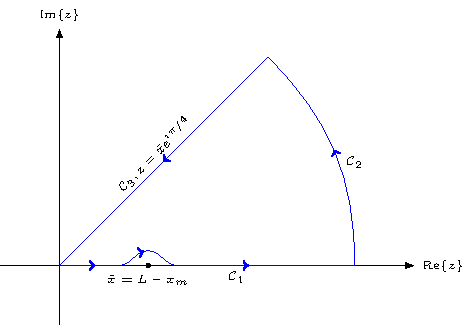
\includegraphics[width=5in]{../media/path_contour-figure0.pdf}
  \end{center}
  \renewcommand{\baselinestretch}{1} \small\normalsize
  \begin{quote}
    \caption[Path Contour]{ Path Contour\label{mp_fig:6}}
  \end{quote}
\end{figure}
\renewcommand{\baselinestretch}{2} \small\normalsize

To ensure we take the path of steepest descent, we can transform $\tilde{x}$ to the complex variable $z$ by applying a phase shift of $\pi/4$. Now we can approximate the integral as

\begin{equation}
\begin{gathered}
I = -2\int_{\mathcal{C}_3}d\tilde{z}e^{i\pi/4} \frac{\Gamma(x_m)}{\Gamma_1}\exp\left[\frac{-kL_0''}{2}\tilde{z}^2\right]  \\
= 2e^{i\pi/4}\int_{0}^{\infty}d\tilde{z}\frac{\Gamma_1}{\Gamma_1}\exp\left[\frac{-kL_0''}{2}\tilde{z}^2\right]  \\
= 2e^{i\pi/4}\sqrt{\frac{2\pi}{kL_o''}}
\end{gathered}
\label{mp_eq:25}
\end{equation}

This yields an asymptotic approximation for the deterministic component of equation \ref{mp_eq:21}.
\begin{equation}
\boxed{F_p = e^{ikL_1} +2\Gamma_1 e^{i\left(kL_{so} + \pi/4\right)}\sqrt{\frac{2\pi}{kL_o''}}}
\label{mp_eq:26}
\end{equation}